\documentclass[12pt]{article}
\usepackage{geometry}                
\geometry{letterpaper}                   

\usepackage{graphicx}
\usepackage[nottoc,numbib]{tocbibind}
\usepackage{amssymb}
\usepackage{epstopdf}
\usepackage{caption}
\usepackage{subcaption}
\usepackage[square, numbers, comma, sort&compress]{natbib} 
\usepackage{amssymb, amsmath}
\usepackage{pdfpages}
\usepackage{hyperref}
\usepackage{listings}
\usepackage{color} %red, green, blue, yellow, cyan, magenta, black, white
\definecolor{mygreen}{RGB}{28,172,0} % color values Red, Green, Blue
\definecolor{mylilas}{RGB}{170,55,241}
\lstset{language=Matlab,%
    %basicstyle=\color{red},
    breaklines=true,%
    morekeywords={matlab2tikz},
    keywordstyle=\color{blue},%
    morekeywords=[2]{1}, keywordstyle=[2]{\color{black}},
    identifierstyle=\color{black},%
    stringstyle=\color{mylilas},
    commentstyle=\color{mygreen},%
    showstringspaces=false,%without this there will be a symbol in the places where there is a space
    numbers=left,%
    numberstyle={\tiny \color{black}},% size of the numbers
    numbersep=9pt, % this defines how far the numbers are from the text
    emph=[1]{for,end,break},emphstyle=[1]\color{red}, %some words to emphasise
    %emph=[2]{word1,word2}, emphstyle=[2]{style},    
}
\usepackage{indentfirst}
\DeclareGraphicsRule{.tif}{png}{.png}{`convert #1 `dirname #1`/`basename #1 .tif`.png}

%\title{Title}
%\author{Name 1, Name 2}
%\date{date} 

\begin{document}


\thispagestyle{empty}

\begin{center}

\includegraphics[width=5cm]{ETHlogo.pdf}

\bigskip


\bigskip


\bigskip


\LARGE{ 	Lecture with Computer Exercises:\\ }
\LARGE{ Modelling and Simulating Social Systems with MATLAB\\}

\bigskip

\bigskip

\small{Project Report}\\

\bigskip

\bigskip

\bigskip

\bigskip


\begin{tabular}{|c|}
\hline
\\
\textbf{\LARGE{Shoe Resale Market Model from Fashion Trends}}\\

\\
\hline
\end{tabular}
\bigskip

\bigskip

\bigskip

\LARGE{Arturas Malinauskas \& David Martinez de la Cruz}



\bigskip

\bigskip

\bigskip

\bigskip

\bigskip

\bigskip

\bigskip

\bigskip

Zurich\\
December 2018\\

\end{center}
\newpage

%%%%%%%%%%%%%%%%%%%%%%%%%%%%%%%%%%%%%%%%%%%%%%%%%

\newpage
\section*{Agreement for free-download}
\bigskip


\bigskip


\large We hereby agree to make our source code for this project freely available for download from the web pages of the SOMS chair. Furthermore, we assure that all source code is written by ourselves and is not violating any copyright restrictions.

\begin{center}

\bigskip


\bigskip


\begin{tabular}{@{}p{3.3cm}@{}p{6cm}@{}@{}p{6cm}@{}}
\begin{minipage}{3cm}

\end{minipage}
&
\begin{minipage}{6cm}
\vspace{2mm} \large Arturas Malinauskas

 \vspace{\baselineskip}

\end{minipage}
&
\begin{minipage}{6cm}

\large David Martinez de la Cruz

\end{minipage}
\end{tabular}


\end{center}
\newpage

%%%%%%%%%%%%%%%%%%%%%%%%%%%%%%%%%%%%%%%



% IMPORTANT
% you MUST include the ETH declaration of originality here; it is available for download on the course website or at http://www.ethz.ch/faculty/exams/plagiarism/index_EN; it can be printed as pdf and should be filled out in handwriting
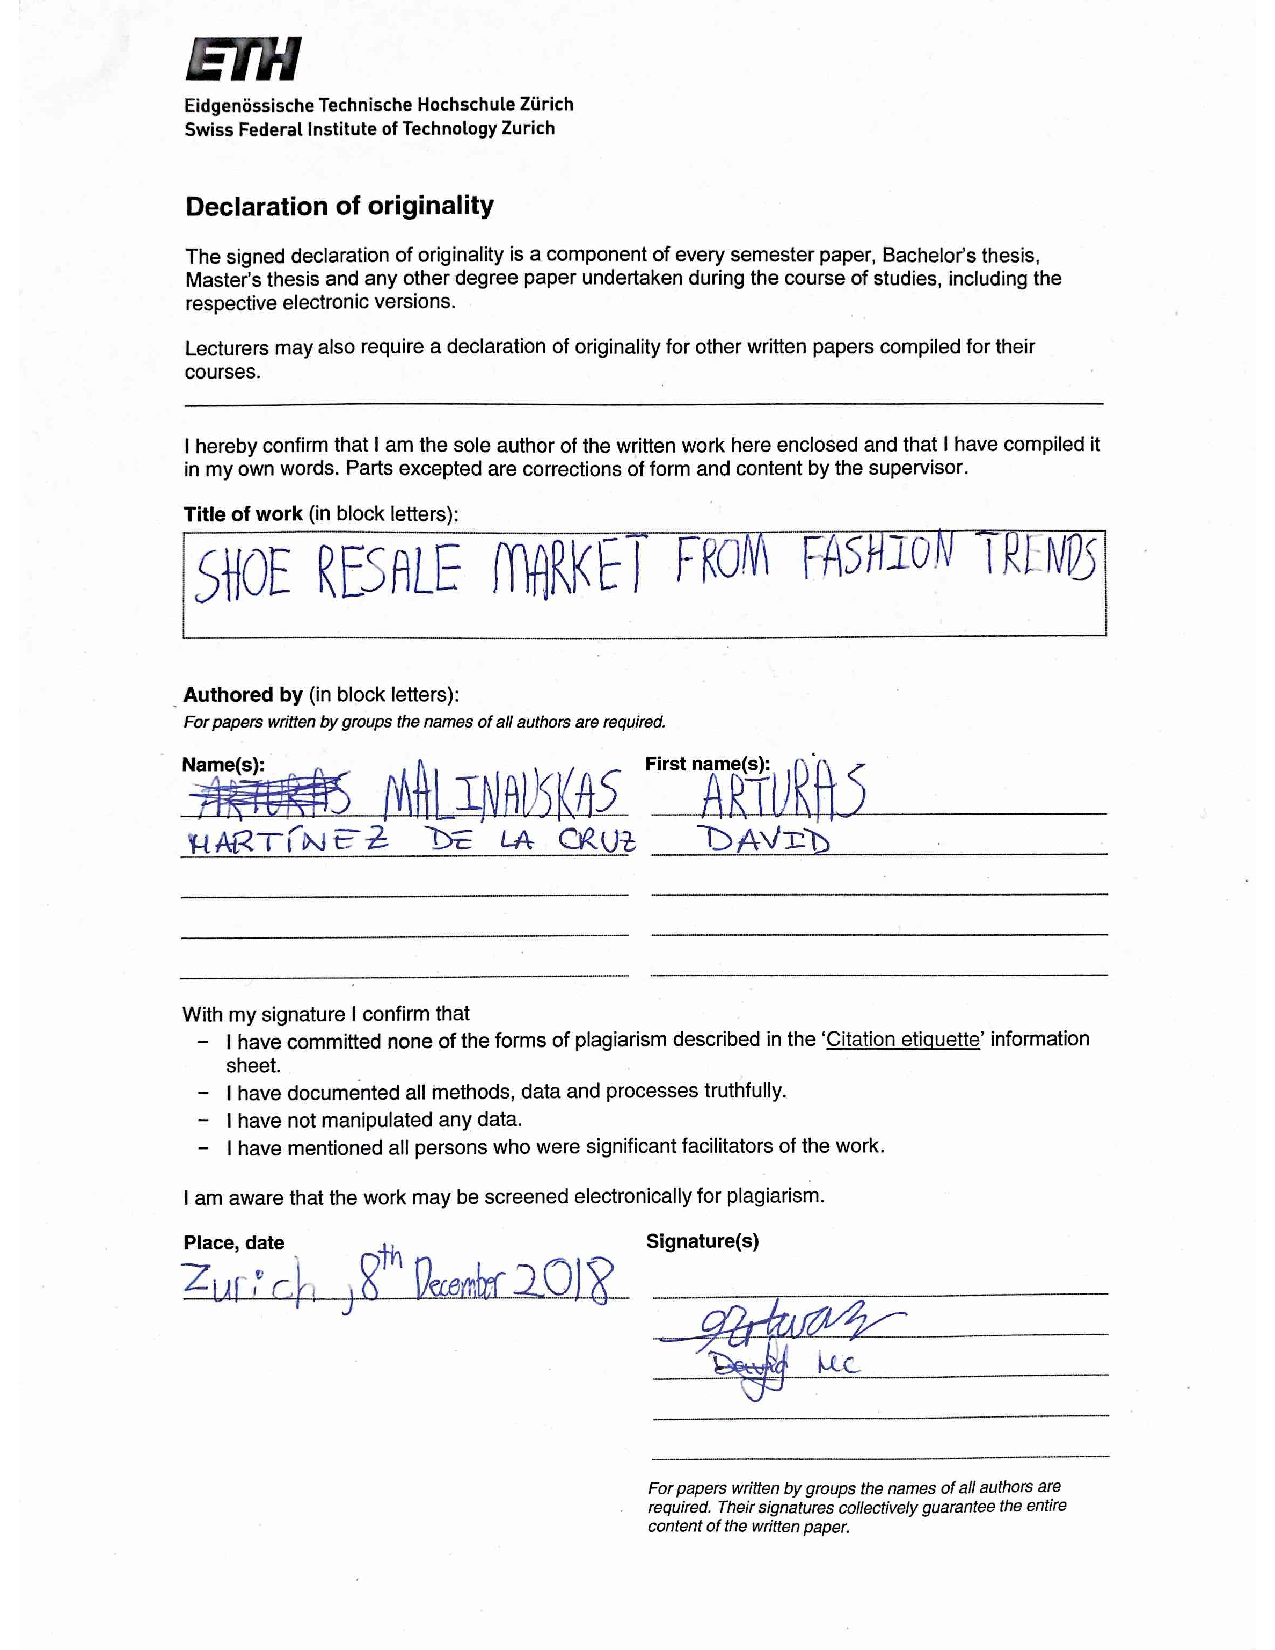
\includepdf[pages=-]{ETH-MSSM-OriginalityDeclaration.pdf}

%%%%%%%%%% Table of content %%%%%%%%%%%%%%%%%

\tableofcontents

\newpage

%%%%%%%%%%%%%%%%%%%%%%%%%%%%%%%%%%%%%%%



\section{Abstract}

A unique secondary market has boomed in the past five years: sneakers and other fashionable apparel are being sold outside retail stores for 150-1000 \% the retail market price. Demand is high for these items of limited quantity which offer social status and a feeling of uniqueness to their owners. This project simulates this market to understand how its dynamics differ from a traditional stock market. A financial model was created in MATLAB to simulate buyers and sellers of shoes with variable prices and social desirability. 

%should add conclusion summary here too

%\newpage
\section{Individual contributions}

Both team members equally developed the research questions, goals of the project, the final report, and presentation. They also worked together to resolve issues in their individual tasks. %David led the development of the Financial market model and model of agents.
%Arturas researched the behaviour of the real market and collected data from online sources with API tools. 


\newpage
\section{Introduction and Motivations}

Shoes have acquired a cultural significance in parts of the modern world. Many shoes manufacturers partner with trend setters to create stylish limited quantity shoe models. In recent years, these shoes have been selling out quickly in the retail market and then resold in a secondary market with markups reaching over 1000 \% \cite{538}. The sum of these transactions is estimated to be over 1 billion US dollars this year \cite{Forbes}.There are many different players in this secondary market. This project seeks to model transactions in the secondary market and identify the best strategy for each type of player.
\subsection{Motivation}

There is a great pool of research on simulating traditional stock markets \cite{Agent_Model, Stock_variation}. We want to see how applicable these techniques are to a market which is relatively new and has not been studied academically. The resale market for sneakers is also features more diverse players than the stock market. Maximizing financial returns is not the only motivation for some people in the sneaker resale market. The sneakers themselves offer a social value from their rarity and style that many people want to own \cite{538}. We believe it is this desire which creates very large fluctuations in market price above initial retail price. The physical condition of a shoe is also important to its value; pristine shoes sell for more than ones that have been worn more.

This market offers some unique challenges for simulation. The social value of a sneaker is dependant on many things, who is promoting them, the brand, the color, the condition, and its rarity. Like old cars, some sneaker models increase in value simply because they are vintage and viewed as "classics" that defined a brand. These factors are not equally valued in the eyes of the different traders in the market. The traders themselves have different incentives: some want to maximize the stylishness of their sneakers, some want to collect the most interesting sneakers (sometimes not even wearing them), and some are simply seeking to profit as middlemen serving the other groups. Some consumer exhibit behavior that is a combination of the previous factors. The various types of traders create a more complicated and perhaps more interesting trading dynamic than the one seen in the stock market.

%All these groups may want to buy the shoes at their initial release. Due to limited quantities, some people use online transaction bots to buy online items faster than any real person could type their information into the system \cite{538}. Other people camp outside stores, sometimes over multiple days, just to be the first ones able to buy a new shoe at its release \cite{538}. 

\subsection{Fundamental Questions}
\label{FundQ}
\begin{itemize}
    \item How does the proportion of sneakers to agents affect price?
    \item How is price affected by the number of competing sneaker brands?
    \item Which market parameters are the most impactful on price?
    \item What behaviors of the sneaker market differ from a standard stock market model?
\end{itemize}

The first question is important to sneaker manufacturers. They decide the number of sneakers they will make and the initial selling price. The manufacturers want to maximize profit. But they receive an intangible benefit to their brand's reputation and desirability due to excitement and promotion in the resale market  \cite{538}. Thus some firms may not sell a shoe for the highest price they could in the present, because they want to create excitement and demand for their brand in the future. Knowing how many sneakers are needed to satisfy a given number of agents would help manufacturers optimize their business.

The second question is important to manufacturers and profiteers. The market has many competitors with limited product differentiation. It is important to understand how competitors may induce price competition.

The third question is important to evaluating price sensitivity. By understanding the most important parameters, the people that are represented by our agents may be able to take information about the real values of those parameters and better inform their own strategies for trading in the market.

The fourth question is important to the academic scope of this work. If there are few differences, it indicates that existing modeling techniques can be applied to a broader array of problem types. If there are significant differences, this opens up new avenues of research to more deeply understand the behavior of non-traditional markets. Appropriately modeling and understanding those different behaviors may offer greater insight into the subtle dynamics of economic systems.

\subsection{Expected Results}
We expect to find that reducing the ratio of sneakers to agents will increase resale price and create more volatility in the market. Lower supply for given demand should create higher prices in accordance to basic economic theory. If there are too few shoes in the market, the agents may not be able to afford them, which would reduce transaction frequency. This would correspond to a loss of excitement over a specific shoe type.

If the sneaker to agent ratio is constant, but there are more competing brands, the prices should also go down. The model gives preference to owning a greater variety of sneaker types for the collectors and socialites. This should result in prices going down as agents are able to bid on a wider variety of products.

We expect the sneaker to agent ratio to have a larger impact on price than the number of competing brands. This parameter affects the available supply. From an economic perspective the available supply should affect price more than the presence of competition. 

There should be some noticeable differences between stock market models and our sneaker market model because our trader agents have behaviors not seen in the stock market. We expect that the different agents see different rates of return based on their preferences for social status or economic value.


\newpage
\section{Description of the Model}

This is a complex market with many dynamics, players, and price factors - many of which are not perfectly rational. So we identified the core elements of the model that lent themselves to computational simulation. We built on previous research by Raberto \textit{et al.} \cite{Agent_Model}
which uses an agent based model to simulate a stock market. 

In Raberto \textit{et al.}'s model \cite{Agent_Model}, the agents are traders who buy and sell stocks. The sneaker market behaves in a similar way with buyers and sellers. The difference is that non-price value of sneakers is modelled as an additional parameter. Thus, the shoes that are bought and sold are represented by two numbers: a price and a "social status". The social status parameter represents the non-price based appeal of the shoe. The social status quantifies how people in the real world would view the stylishness, quality, and condition of a shoe. The agents respond to the social status in different ways and have different end objectives. The four agents we model are the trendsetters, socialites, collectors, and profiteers. 

\subsection{Description of Agents}
The trendsetters are agents that bring shoes into the marketplace. They represent different shoe brands and create the initial social status. As trendsetters they do not need to buy shoes.

The socialites are agents who buy and sell sneakers to optimize social status. These correspond to people in the real world that buy trending sneakers, wear them for a short time, and sell or exchange them for different sneakers.

The collectors are agents who buy but do not sell any sneakers. They correspond to people in the real world that want to buy the best shoes which will retain value. They take shoes out of the marketplace and often display them in personal collections or shoe racks. In the real world, these collectors may also sell some of their shoes, or buy multiple pairs so they can wear some while keeping another pair in pristine condition. Collectors in the real world often have one to two hundred different pairs of shoes \cite{538}

Finally the profiteers are agents who buy and sell sneakers to maximize monetary profit. These agents ignore the social status. These correspond to people in the real world who have little interest in sneakers themselves, but want to capitalize on high mark ups over retail price.

There are many other types of agents that could have been modelled, but the complexity of their addition did not justify their lesser importance to the market. For example, individuals in the real world may switch roles based on their own incomes and personal impulses. There are counterfeit shoes in the market, scammers who take people's money without sending anything in return, trading bots, and other miscellaneous occurrences that happen less frequently than the core behaviors we modelled.

When modeling the agents, each of them will have different properties which will differ from one type of agent to another. This fields include the social status of the agent, which varies over time; the desire to buy new shoes, defined depending on the agent; and some initial money to start trading.

These agents are classified into buyers and sellers, depending on their type and several factors. Socialites will become sellers if they do not have more money to buy and they have some items, or if they do not want to wear their sneakers anymore. Profiteers however, become sellers when the average value of their assets is higher than the average selling price of the market, trying to maximize their profit. Whenever these two agents sell all their items, they become buyers again.

\subsection{Trading Environment}
\label{Env}
The environment for the agents is a closed market, where the items are released by the trendsetters and then interchanged between the different agents according to their needs and desires. The agents are fixed, meaning they don't change from one type to another and there is no exit or entry of agents into the market. The shoes being traded may depreciate in value to a point where they are no longer sold in the market. But new shoes will be periodically released into the market to ensure demand is met. It is also assumed the agents have supplemental sources of income which is paid out regularly in set periods (representing their real world salary from a job). This ensures that new items in the market are affordable by some people.

The market operates at every time step, which corresponds to a day of trading. Buyers and sellers will decide their individual prices for a day of trading. Buyers that are unable to buy shoes during a trading day will generally increase the price they are willing to pay on the next day. Sellers that are unable to sell a shoe at a price will generally decrease the price they are willing to pay. The time it would take to ship sneakers from buyers to sellers is ignored. 

The transactions only occur when certain conditions are met. These conditions depend on the buying price of each buyer and the selling price of each item. The former has to be higher than the latter for the transaction to take place. Additionally, the social status of the item is tied to a random variable. Sneakers with less social status are less likely to be sold in the market. 

\newpage
\section{Implementation}
\subsection{Inputs}

The inputs required by the user to run this simulation are mainly associated with the size of the simulation. The number of agents to be simulated and the amount of sneakers introduced in the market have to be set. In order to simulate the behaviour of this market, the model should be run with a larger number of agents than items sold. If this is not true the economic system breaks down because the items are no longer limited, everyone could buy one. This is true for the real world: there are many more people interested in buying the limited edition shoes than the available supply of those shoes. The scarcity creates value in all economic systems.

Furthermore, an initial price for the buyers needs to be set. This sets an initial condition and only affects the buying prices in the beginning of the simulation. The buying and selling prices are modified later depending on offers and demand.

The last inputs required are the amount of brands for the sneakers and the duration of the simulation, which is given by the days the user wants to simulate. The former input has to be reasonable according to the amount of agents introduced in the system and the amount of items. 

With these inputs set, the model is set to run and simulate the evolution of the model explained in the previous section.

\subsection{Outputs}

The outputs produced by the program are a set of graphs showing the evolution of different parameters through time as well as some final characteristics that define the agents and their behaviour. These graphs and figures will be discussed in the following section \ref{Sim_Dis}.

\subsection{Fixed Simulation Parameters}

For the simulation to run more parameters than the ones provided in the input routine are needed. These values are set in the code, and they can either have a fixed value during the whole simulation or vary randomly as time goes on. The frequency with which brands release new sneakers to the market is set to be one of those random values calculated in the code, as well as the change in social status of the items through time. The fixed values include for example how much the buying and selling prices are increased or decreased depending on whether the agent performed a transaction or not. These values are weighted with the desire of the buyers to buy the items.

These parameters have been optimized in the code through many iterations so that the model represents the real behaviour of the market and doesn't produce results far from examples we found in our research. This optimization allowed us to better understand the important market dynamics and critically think about why values had to be in certain ranges.

\subsection{Code Structure}
In the code's first steps, the data structures are created and initialized. There are two main data structures, buyers and sellers, which are then selected to be one of the agents described previously. Initially only trendsetters are sellers, as they are the ones to introduce the sneakers into the market. Then the rest of the agents become potential buyers.

Each buyer is then assigned a set of attributes corresponding to their initial money, social status, and desire to buy items. Sellers on the other hand are assigned assets which are assigned randomly to one brand. A check is made to ensure each brand is represented by a trendsetter. Each brand is then assigned a random social status and initial price, which transfers to the trendsetters belonging to that brand. This way the items get their initial selling prices and social value.

Before running the simulation, some parameters are initialized, such as the increase or decrease in prices depending on the transaction. The code starts the simulation, which performs the purchase of the item, the change in the agents' attributes according to their actions and the update of the items social status as time progresses.

The first lines of the loop for the simulation calculate all the desired information in each iteration, such as the average selling price or the average buying price of each different type of agent. Then the trading operation between the agents occurs. Transactions happen only when the conditions mentioned in subsection \ref{Env} are fulfilled. With the purpose of approximating reality, the constraint that one buyer can only buy one item per day has been applied into this model. 

The next lines in the code (shown in \ref{AppA}) vary the different parameters associated with each agent. For buyers, the buying prices are adjusted, the social status is calculated based on the items they own, and the desire changes depending on their agent type. Sellers lower their selling prices if they did not manage to sell one item. 

Following these changes, the agents are moved from buyers to sellers and the other way around according to the factors explained before. Both sellers and buyers retain their values for desire, social status, buying price, etc, as they are the same people that move from one side to the other of the market.

Finally, the status of the items is changed in each iteration. Due to depreciation, items lose a random amount of their social status, making it less likely to be bought. This also accounts for the loss of value because of wear. Each brand is also assigned a factor equating to 'vintageness', so some shoe brands increase in social status. However, depreciation tends to be bigger in our time scales and the social status of the shoe decays in time.

Once all of this actions are performed, the new day begins with the transactions between the new buyers and sellers according to their new parameters.


% In order to perform the buying and selling operations, each sneaker is given a starting selling price based on the social status of the item. The higher the social status, the higher the selling price will be. On the other hand, agents are given a certain amount of money, depending on their desire to buy the sneakers. This desire is set different for each agent, as they have different goals. While socialites try to maximize their social status, profiteers try to increase their initial amount of money, and thus their desires will vary differently along time. Socialites have a 50% chance of becoming sellers at each time step. This corresponds to a person that gets bored or wants new shoes due to their own impulses.

% Once the shoes and the agents are modelled, the environment in which agents develop their activities is set. Sellers act on their item's prices depending on whether they are bought or not and buyers modify their buying prices according to their transaction. Furthermore, the factors of depreciation and 'vintagness' are introduced in the model, making the social status of the item change through time. This social status affects also the owner, whose social status increases or decays with the different purchases. 

\newpage
\section{Simulation Results and Discussion}
\label{Sim_Dis}

To answer the fundamental questions proposed in subsection \ref{FundQ}, several simulations have been carried out. The different simulations varied the input parameters to test the most influential parameters.

\subsection{Nominal Test}

We perform a baseline simulation which is used as a comparison for our results. The parameters of the baseline are conservative values that ensure the model is stable. The results from this simulation are our reference for further runs and changes to the input parameters. 

The number of agents chosen for this simulation is \textit{N = 1000} with \textit{$n_{items} = 800$} which will be divided into 4 different brands, which will be initialized randomly. The starting price for the buyers in this market is \textit{p = 700} currency units. This market will be modelled for one year, so the time steps for the iteration will be \textit{t = 350} days. 

The following graphs illustrate the results obtained with this simulation. In \textit{Figure} \ref{Avgp_Nom} the average of the buying prices from all the different agents and the global average of the selling price. It can be seen the different strategies followed by each type of agent. The buying prices from the socialites and profiteers do not present much difference from one another. They interchange the roles of sellers and buyers once all the items have been released to the market by the trendsetters. As it can be seen, the socialites are the more active in the market, with a buying price closer to the average selling price.

\begin{figure}
    \centering
    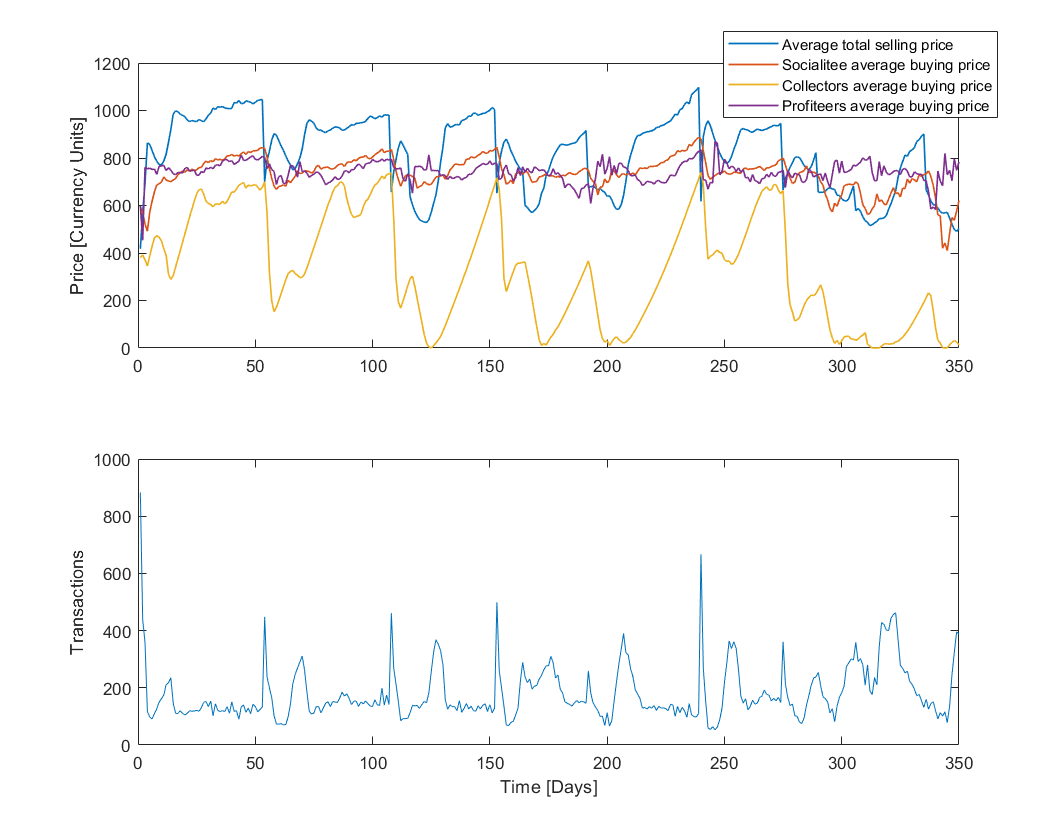
\includegraphics[width=0.6\columnwidth]{Nominal_Out/Avrg-prcs2nom.png}
    \caption{\textbf{Top} - Average buying prices from the different buyers and global average price. \textbf{Bottom} - Number of transactions each day. Simulation ran with \textit{N=1000}, \textit{$n_{items}=800$}, \textit{$n_{brands}=4$} and \textit{t=350 days}}
    \label{Avgp_Nom}
\end{figure}

Meanwhile, the collectors follow a very different trend. These agents buy during the first day of the new items, as this items are the ones worth to collect. This makes them run out of money, and therefore their buying prices decay and start rising, as they earn money through time. When new items are introduced, they use this money in order to acquire the brand new released sneakers

Furthermore, the average selling price is higher than the average buying price. This corresponds to the real world, where no seller wants to sell for less of what the paid to buy the item. The only points in which the selling price is lower than the buying price is at very selected days, which correspond with the moments when new items are released. This new items have much lower prices than the value of the sneakers already in the market. It is interesting to note how profiteers increase their buying prices during these periods in order to buy more and therefore sell it for a higher price.

\textit{Figure} \ref{Avgp_Nom} also shows the number of transactions in each day. The peaks shown in this graph correspond to the moments when new items are released and when they are starting to get sold in the market as socialites get tired of them and go looking for different sneakers. As time progresses, more items are in the market and the number of transactions starts oscillating at the end of the simulation run. This because there are more items to be interchanged and the agents are more active, trading more goods.

The introduction of new items to the market can be observed in \textit{Figure} \ref{Avgtim_Nom}. This graph also shows how newer items have a higher selling price, as they are more demanded. The last two graphs show also how the selling price of the items introduced in one period increases during that period until new sneakers are introduced. This is because items start coming out of the market as they have a social status below a certain threshold, or they are property of the collectors, being also out of the market.

\begin{figure}
    \centering
    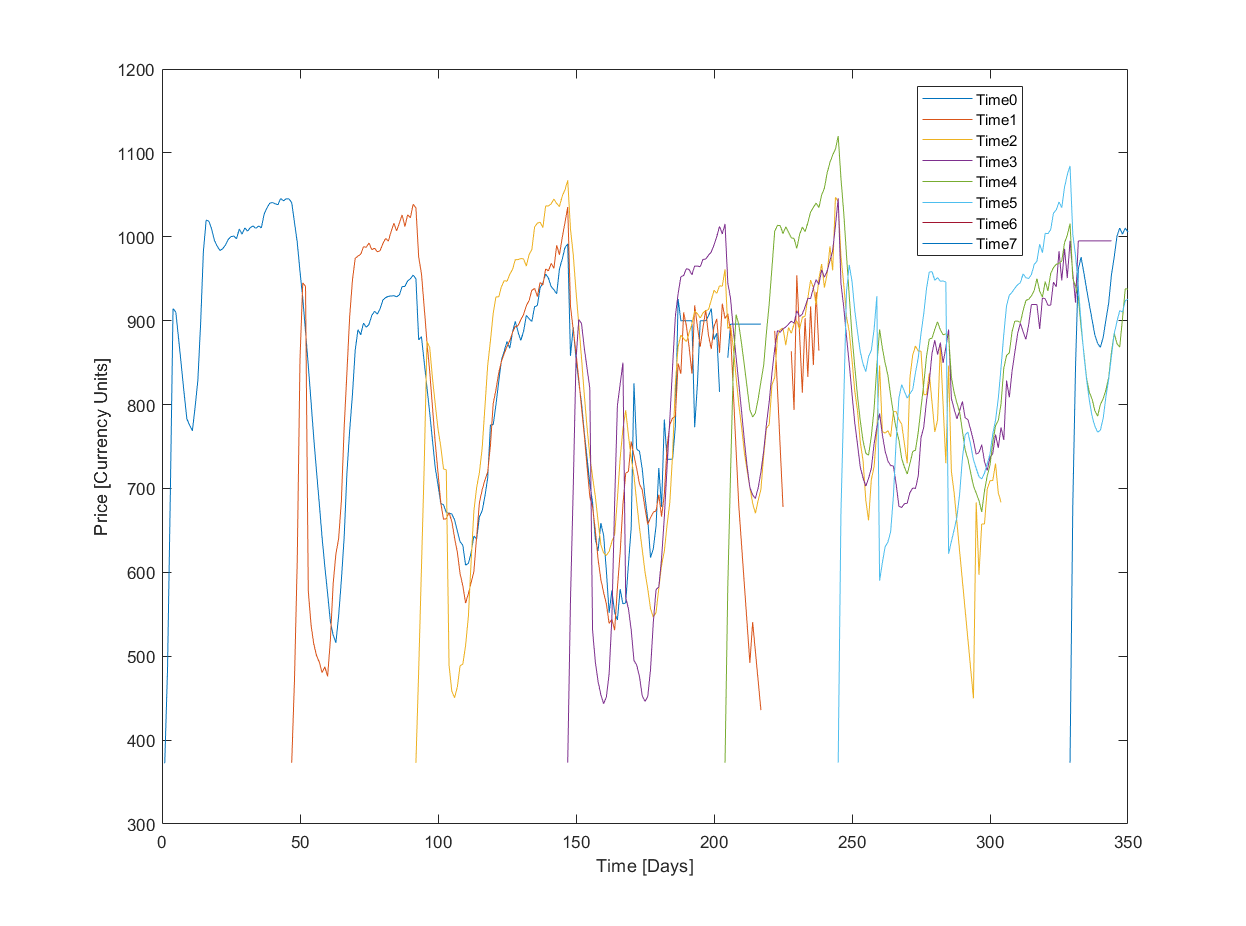
\includegraphics[width=0.6\columnwidth]{Nominal_Out/timepnom.png}
    \caption{Average selling price of the items introduced in each time period. Time0 being the oldest items in the market and Time7 the newest. Simulation ran with \textit{N=1000}, \textit{$n_{items}=800$}, \textit{$n_{brands}=4$}, \textit{p=700} and \textit{t=350 days}}
    \label{Avgtim_Nom}
\end{figure}

Another interesting result to look at how the different brands evolve through time. This brands are affected by the depreciation and by a random 'vintageness' factor, which is equal for each brand but it is created randomly every iteration. The result of this behavior can be seen in \textit{Figure} \ref{Avgbrnd_Nom}. This graph shows how competitive this market is, where the four different brands have a similar buying price. However, the best-selling brand changes from time period to time period. This reflects the reality, as different designs and models from the same brand have a bigger or smaller impact on society. When looking through a sort period of time, it can be seen how 'vintageness' affects randomly to the brands, as their selling prices oscillates within days.

\begin{figure}
    \centering
    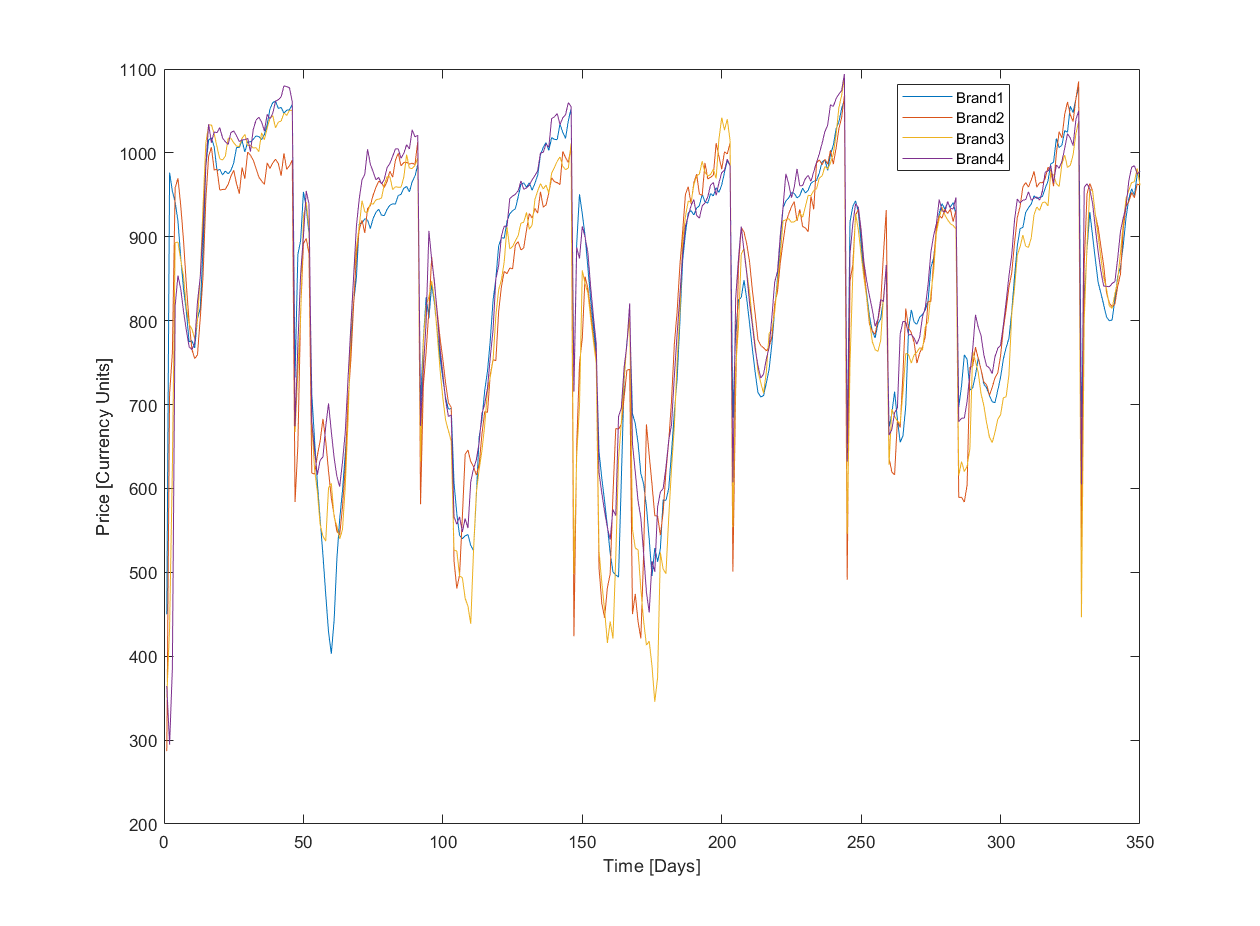
\includegraphics[width=0.6\columnwidth]{Nominal_Out/brndpnom.png}
    \caption{Average selling price per brand. Simulation ran with \textit{N=1000}, \textit{$n_{items}=800$}, \textit{$n_{brands}=4$}, \textit{p=700} and \textit{t=350 days}}
    \label{Avgbrnd_Nom}
\end{figure}

The results of these transactions in the market can be seen in \textit{Figure} \ref{profitnom}, where the net profit of the profiteers can be seen. This profit is calculated as the difference of what they paid for the items and what they sold it for. When the market closes, the value of each profiteer's inventory is added, as this is money they have invested. However, this leads to some error, as for profiteers who are still buyers, they are selling it for a lower price and therefore losing money, which would not be the behavior of the modelled profiteer. 

\begin{figure}
    \centering
    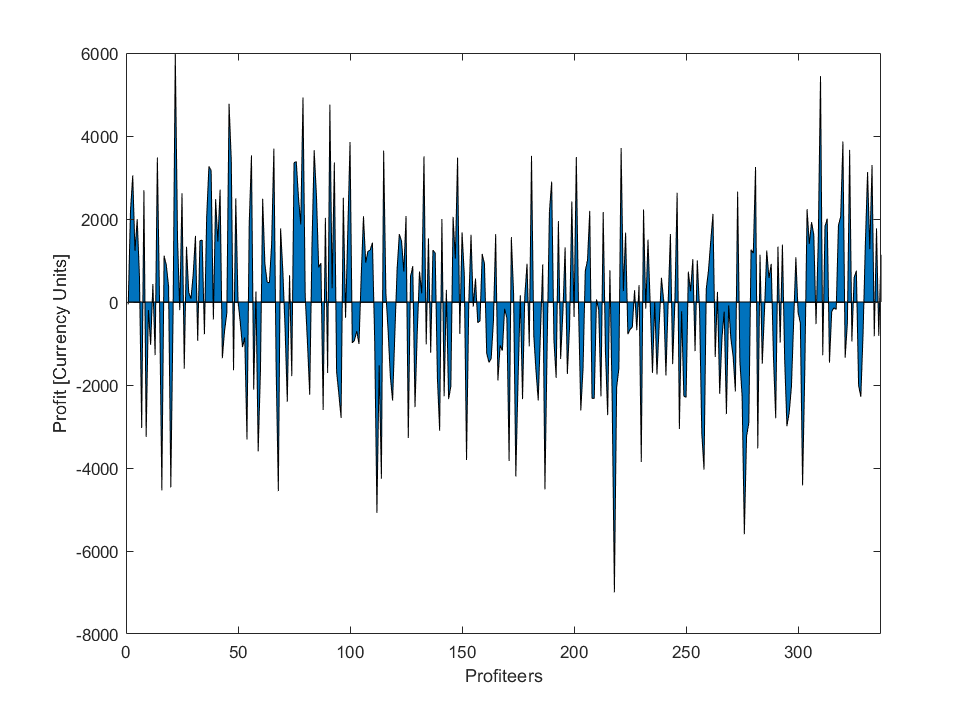
\includegraphics[width=0.6\columnwidth]{Nominal_Out/profit_nom.png}
    \caption{Profit made by each profiteer at the end of the simulation. Current inventory is added. Simulation ran with \textit{N=1000}, \textit{$n_{items}=800$}, \textit{$n_{brands}=4$}, \textit{p=700} and \textit{t=350 days}}
    \label{profitnom}
\end{figure}

\vspace{5cm}

These results from the nominal inputs can be now used to analyze how the outputs of the market vary when changing the inputs and therefore answer the fundamental questions.

\subsection{Effect of Ratio of Sneakers to Agents}
\label{effrat}

To answer the first question, the following simulation was done. The number of agents was kept constant, \textit{N=1000}, the number of brands \textit{$n_{brands} = 4$} and the initial price \textit{p=700} were the same and the brands were initialized randomly, but the number of items was reduced from 800 to \textit{$n_{items}=200$}. This way, there are not enough items to satisfy all the agents and the competition between them increases. Additionally, the simulation lasted only \textit{t=150} days, as the difference can already be seen in this short period of time and the evolution of the market in time would follow the same trends as in the beginning of it. Similar simulations were performed where the 10:2 ratio of agents to items was retained, but their magnitude varied, using \textit{N=8000} and \textit{$n_{items}=1600$} for a larger number of agents and using \textit{N=100} and \textit{$n_{items}=20$} to simulate fewer agents. The overall behavior was the same in these cases, differing only as expected due to the random parameters.

The first results of this simulation can be seen in \textit{Figure} \ref{avgplow}. These graph shows the comparison between the nominal and this case of the evolution of the average of the buying and selling prices. Comparing these graph with \textit{Figure} \ref{Avgp_Nom}, it can clearly be observed that the prices are much higher when the number of items decreases. As said in the expected results, this is what should happen in an environment where supply is strictly limited and the demand is high. The number of transactions is also displayed. This value is significantly lower, as the number of items available is lower and their prices are much higher, meaning not everyone can afford it. 

\begin{figure}
\begin{subfigure}{0.5\textwidth}
    \centering
    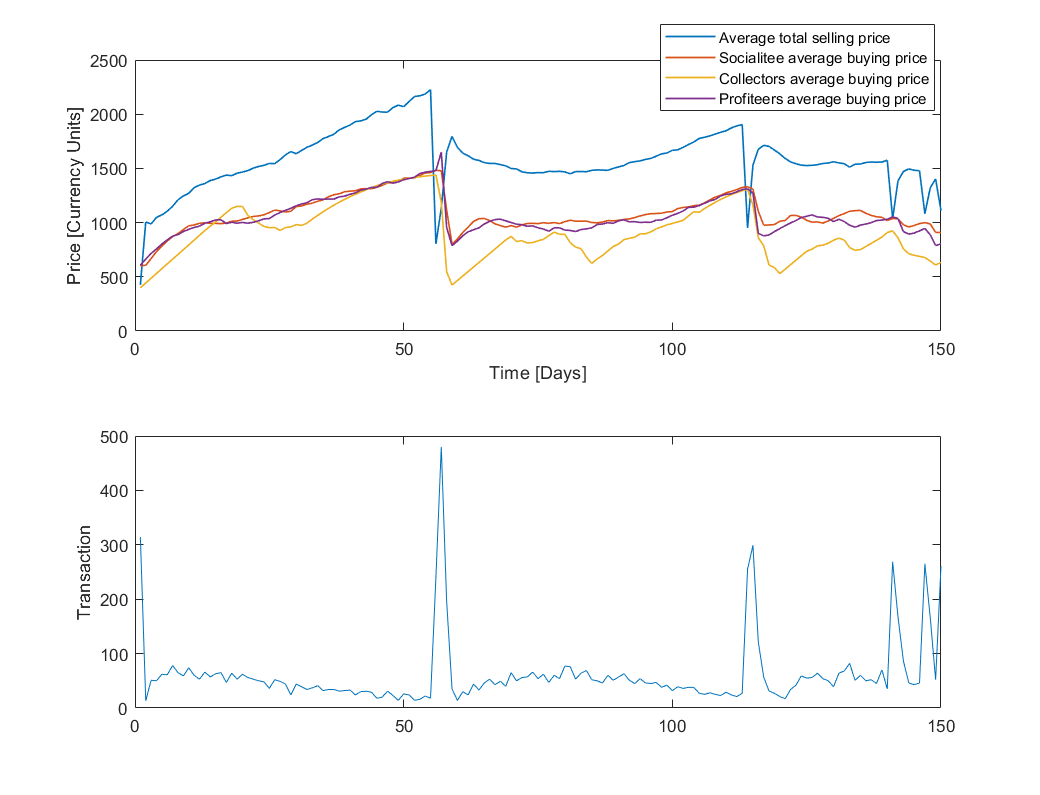
\includegraphics[width=\textwidth]{Low_Items/Avrg-prcs2_lowitems.png}
    \caption{\textbf{Top} - Average buying prices from the different buyers and global average price. \textbf{Bottom} - Number of transactions each day. Simulation ran with \textit{N=1000}, \textit{$n_{items}=200$}, \textit{$n_{brands}=4$}, \textit{p=700} and \textit{t=150 days}}
\end{subfigure}
\begin{subfigure}{0.5\textwidth}
      \centering
    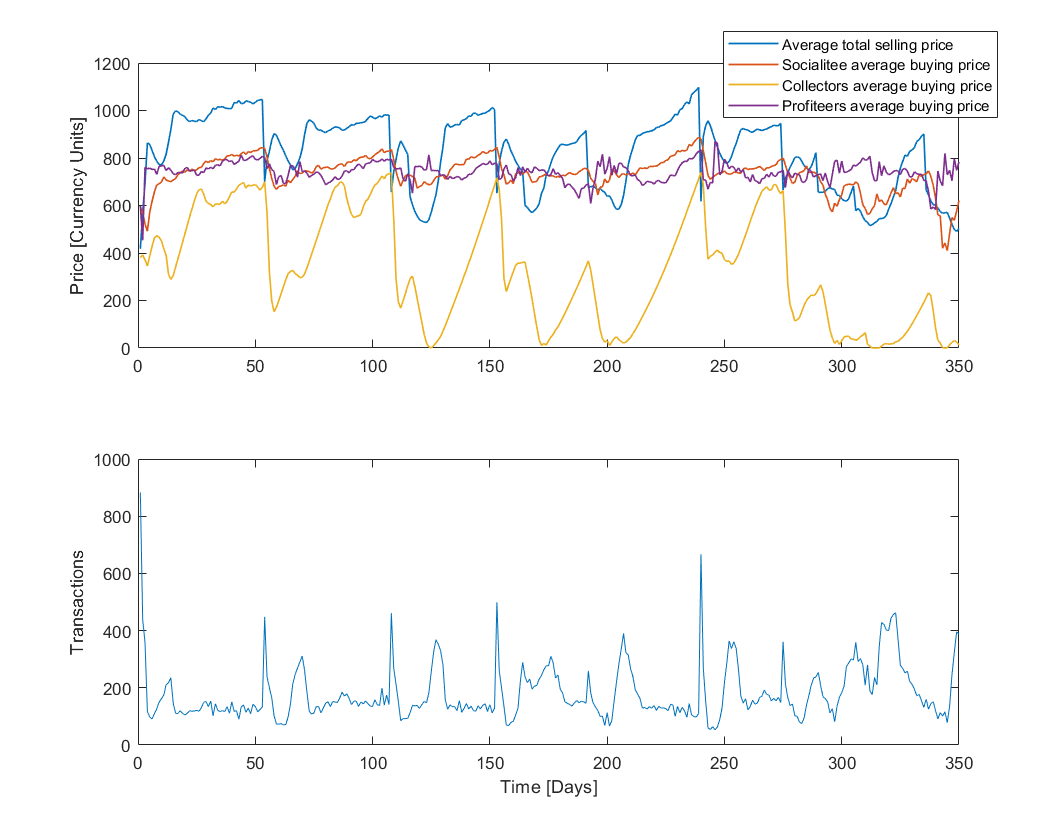
\includegraphics[width=\textwidth]{Nominal_Out/Avrg-prcs2nom.png}
    \caption{\textbf{Top} - Average buying prices from the different buyers and global average price. \textbf{Bottom} - Number of transactions each day. Simulation ran with \textit{N=1000}, \textit{$n_{items}=800$}, \textit{$n_{brands}=4$} and \textit{t=350 days}}
\end{subfigure}
\caption{Comparison between the different values of prices and number of transactions for the nominal case and the low amount of items case}
\label{avgplow}
\end{figure}

This difference is more clearly seen in \textit{Figure} \ref{translow}. The average transaction prices of each day are represented in this graph for both cases, nominal and low amount of items.

\begin{figure}
    \centering
    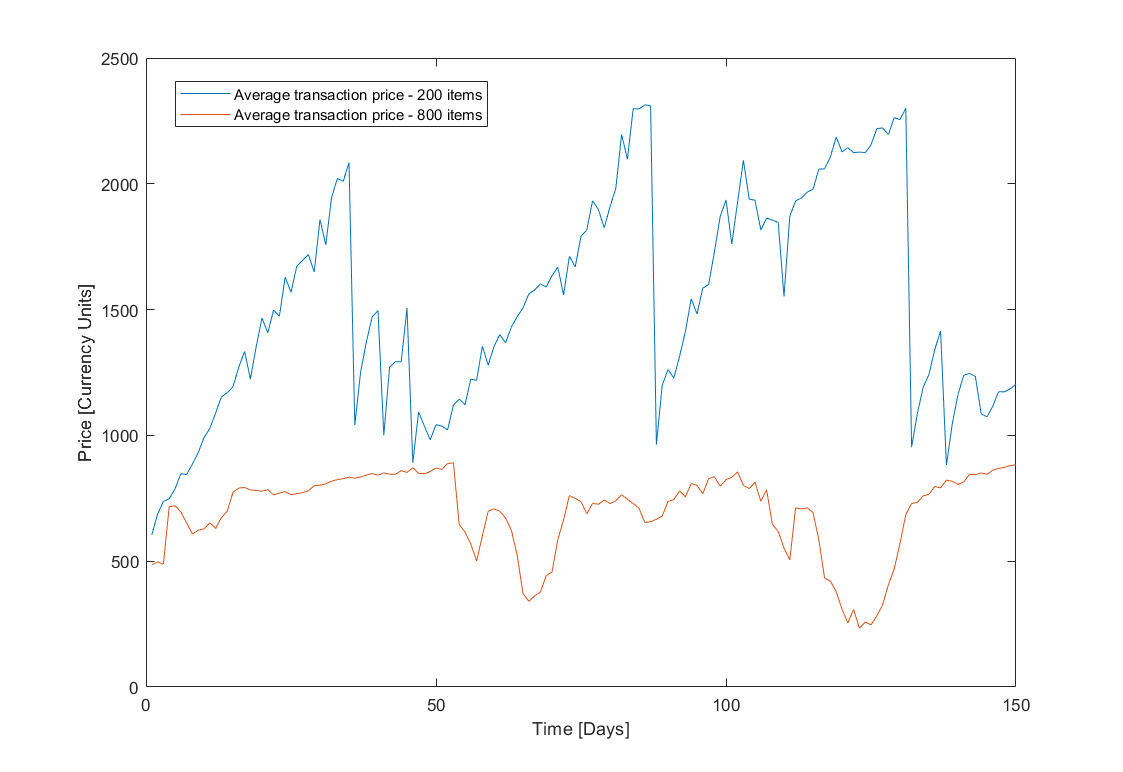
\includegraphics[width=0.6\columnwidth]{Low_Items/Avrg-transp_lowitems.png}
    \caption{Comparison of average transaction prices per day for both cases: \textit{$n_{items}=800$} and \textit{$n_{items}=200$}. Simulation ran with \textit{N=1000}, \textit{$n_{items}=200$}, \textit{$n_{brands}=4$}, \textit{p=700} and \textit{t=150 days}}
    \label{translow}
\end{figure}

\subsection{Effect of Number of Brands on the Price}

This simulations investigates how the agents behave when there are many brands to choose from with different attributes. In this case \textit{$n_{brands}=10$} and all other parameters are the same  as the nominal case. This implies that the simulation cannot be with 100 agents any longer, as this would lead to too few trendsetters and some brands would end up with no representation in the market and would not release their items. Therefore, the number of agents is set to be \textit{N=2500}. As the number of agents increases, so has to do the number of items, or the model would have the same behavior as in the last study. Thus, the number of items in this study is \textit{$n_{items}=2000$}. The rest of parameters are the same as the study in subsection \ref{effrat}. 

The following figures show the behavior of the market under these conditions. \textit{Figure} \ref{compavgbrands} illustrates the comparison between the nominal case and the case discussed in this section. The prices seen in \textit{Figure} \ref{avgbrands} are very similar to the ones obtained for the nominal case. This is implies that the amount of brands does not have a big impact on the price, a result that was expected as the ratio of items and agents has been kept constant. Competition between brands is not a big factor to take into account for the agents. 

\begin{figure}
\begin{subfigure}{0.5\textwidth}
    \centering
    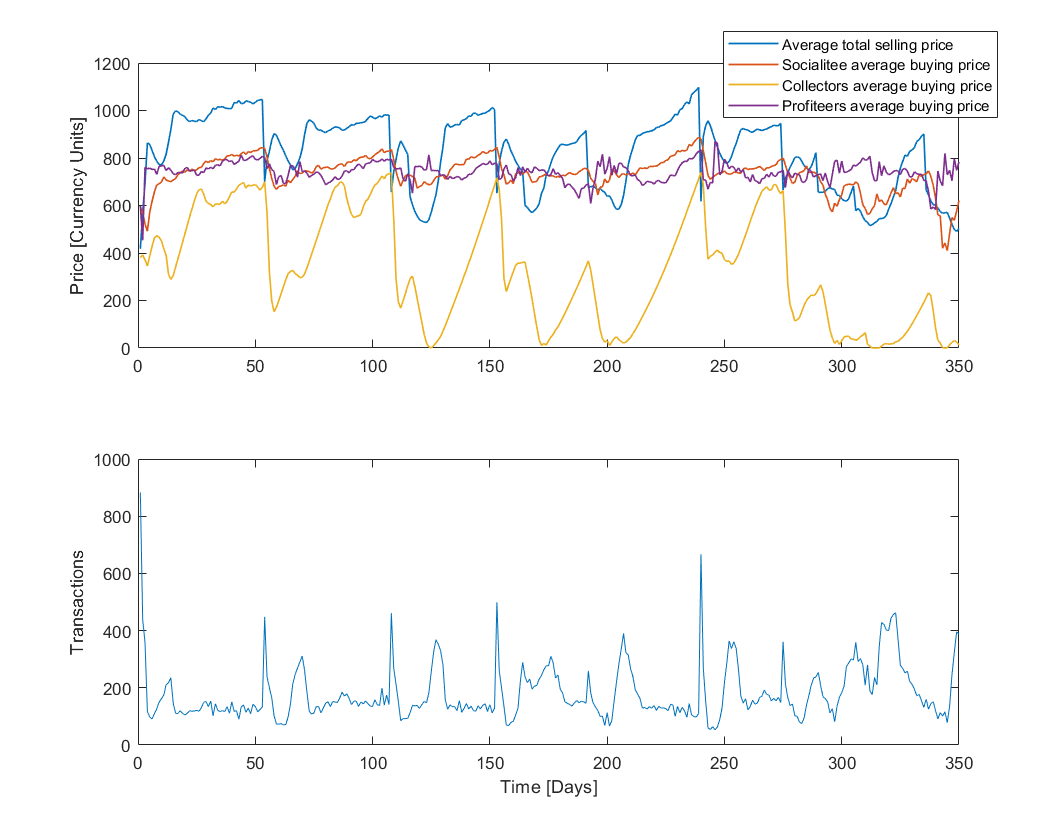
\includegraphics[width=\textwidth]{Nominal_Out/Avrg-prcs2nom.png}
    \caption{\textbf{Top} - Average buying prices from the different buyers and global average price. \textbf{Bottom} - Number of transactions each day. Simulation ran with \textit{N=1000}, \textit{$n_{items}=200$}, \textit{$n_{brands}=4$}, \textit{p=700} and \textit{t=150 days}}
\end{subfigure}
\begin{subfigure}{0.5\textwidth}
      \centering
    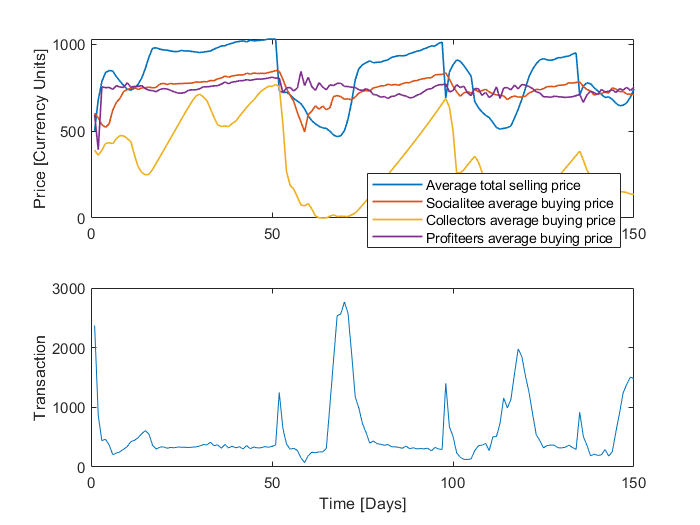
\includegraphics[width=\textwidth]{Brands/Avgp_brands.png}
    \caption{\textbf{Top} - Average buying prices from the different buyers and global average price. \textbf{Bottom} - Number of transactions each day. Simulation ran with \textit{N=2500}, \textit{$n_{items}=2000$}, \textit{$n_{brands}=10$} and \textit{t=150 days}}
    \label{avgbrands}
\end{subfigure}
\caption{Comparison between the different values of prices and number of transactions for the nominal case and the high number of brands case}
\label{compavgbrands}
\end{figure}

However, and as shown in \textit{Figure} \ref{comppbrands}, there is a bigger variance between the prices for each brand. This is also expected, as more brands would lead to more options when buying and the depreciation factor and 'vintageness' feature affects differently each brand and shoe. More difference would be seen if there was a bigger difference between brands, but this would involve modelling several parameters of the brands, which is not the objective of this work and it would increase greatly the complexity of the model.

\begin{figure}
\begin{subfigure}{0.5\textwidth}
    \centering
    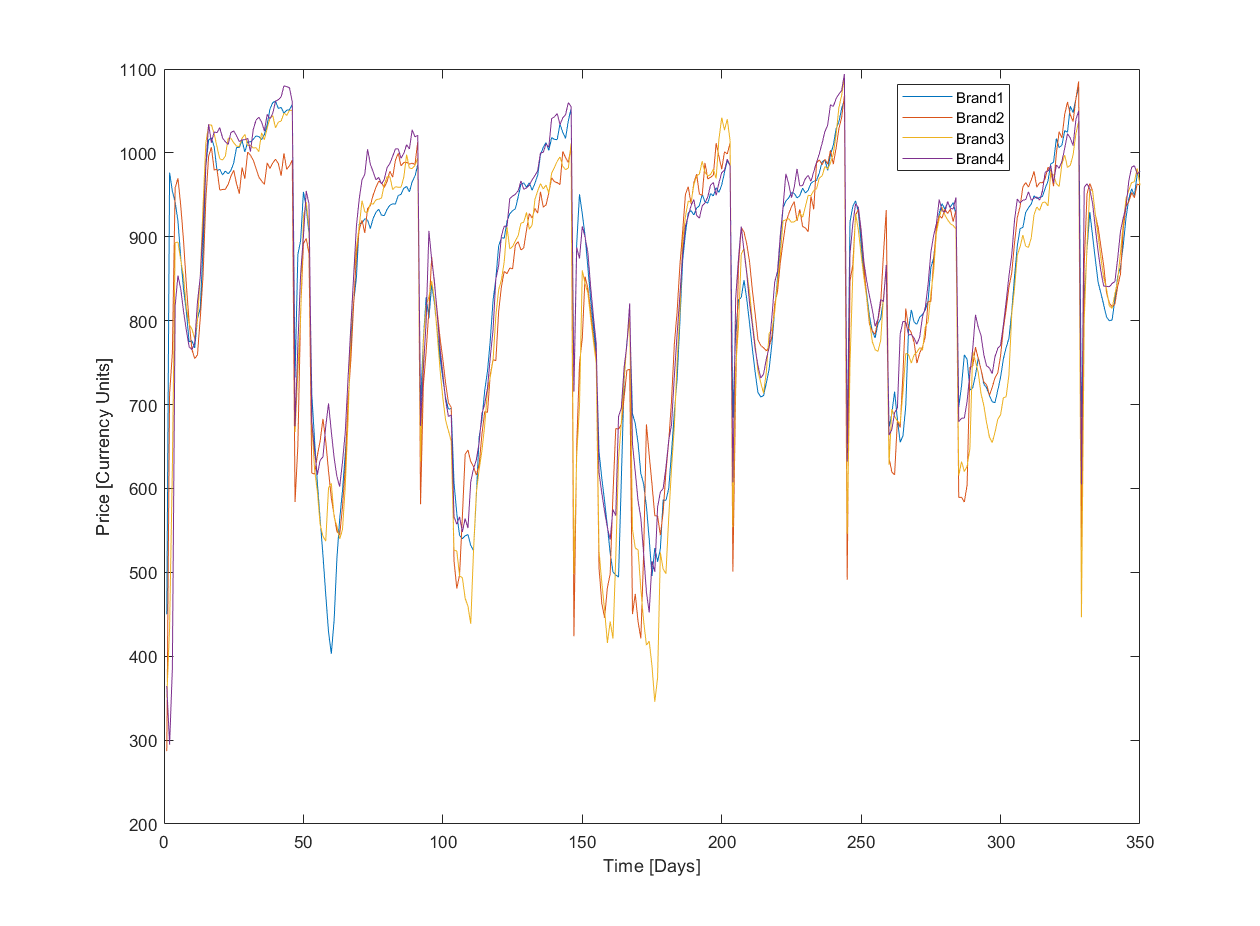
\includegraphics[width=\textwidth]{Nominal_Out/brndpnom.png}
    \caption{Average selling price per brand. Simulation ran with \textit{N=1000}, \textit{$n_{items}=800$}, \textit{$n_{brands}=4$}, \textit{p=700} and \textit{t=350 days}}
\end{subfigure}
\begin{subfigure}{0.5\textwidth}
      \centering
    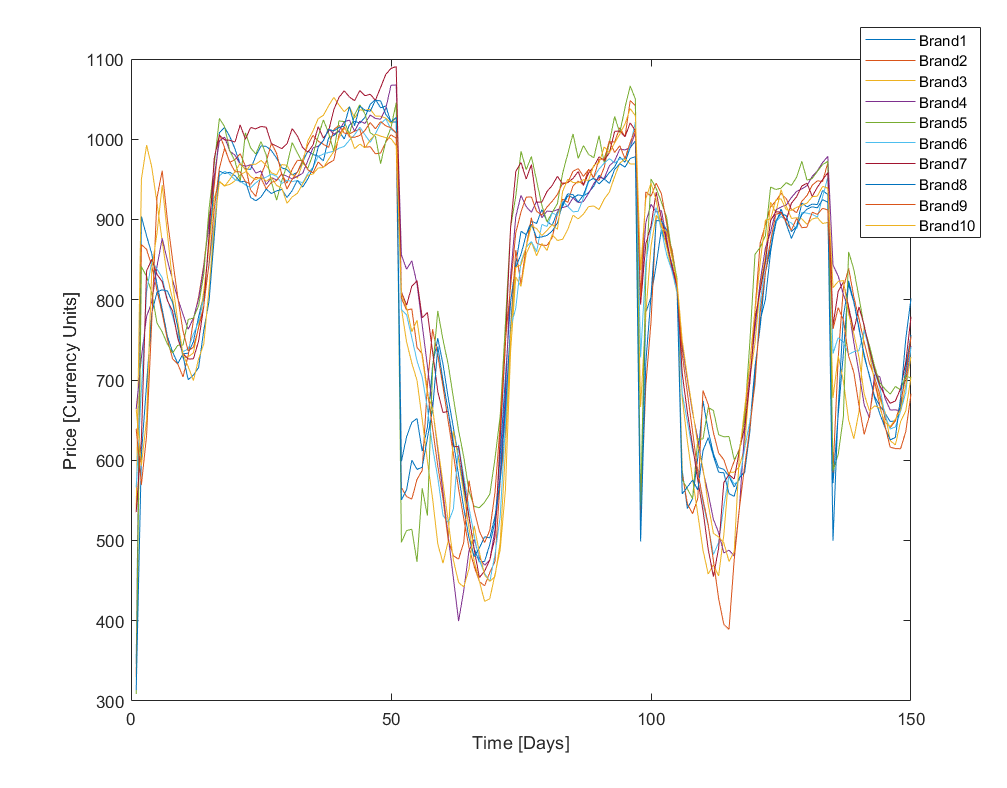
\includegraphics[width=\textwidth]{Brands/Brnd-hbrands.png}
    \caption{Average selling price per brand. Simulation ran with \textit{N=2500}, \textit{$n_{items}=2000$}, \textit{$n_{brands}=10$}, \textit{p=700} and \textit{t=150 days}}
    \label{avgbrands}
\end{subfigure}
\caption{Comparison between the selling prices for each brand for the nominal case and the high number of brands case}
\label{comppbrands}
\end{figure}

\subsection{Most Influential Parameters}

Once these factors have been analyzed, it is clear to see that the amount of items released in the market is a great way to modify the behavior of it. This is of great value to the sneakers brands, which can adapt the amount of items released in order to increase the selling price but without selling any item. Having a surplus of items in the market would also lead to a different behavior than the one presented in this approach, but it would not have a negative impact on the consumers, as the market would be saturated with items and there would be no competition between the agents in order to achieve their desires. 

The initial price of the buyers would have a minor effect in the beginning of the simulation, as it would change the initial amount of assets bought if it was below the selling price, which would not represent the reality, since socialites, profiteers and collectors want to buy first hand items for their own goals. Nevertheless, the influence would decrease as time goes by, reaching the same results explained in this report. 

Another important parameters that have an effect in the market are more intrinsic parameters such as the price variation of the items depending if they are being sold or bought, depreciation and 'vintageness', inflation if the simulation time was over years, etc. However, modifying these parameters would change the behavior of the model, making it less approximate to reality. Therefore, even though these values affect largely the model, they are not values that should be changed from one simulation to another.

\subsection{Difference between Stock Market and Retail Shoe Market}

The big difference between these two markets is the effect of personal value of the items and their intangible value. This value is what is accounted for in the social status term in this model presented, where the value of the shoe not only depends on the time it has been in the market, but who owns it and who released and made that sneaker. Therefore, the shoe retail market has much more factors that could influence a potential buyer or seller.

This is what makes it much more difficult to model and simulate, as it needs to take into account parameters that cannot be expressed by any number or analytic expression. The approximation made in this model is quite simple but reflects the core of this human aspect of the market, giving a vague idea of how this influences the prices and transactions.

\newpage
\section{Summary and Outlook}

The initial results of our simulation show interesting behavior worthy of further study. There are many potential refinements to the code that could increase its accuracy and computational efficiency.  Further research should also be done to incorporate real world data into the simulation. There is a wealth of useful data about consumers in the market on various social media platforms. 

\subsection{Limitations and Simplifications}

Many simplifications had to be made to create this model of the sneaker resale market. The attributes of a variety of different products and people had to be simplified. Fashion is a very subjective topic, which makes objective modeling difficult. Several arbitrary parameters must be made to attempt to model human preferences. 

Due to processing power, we only simulated up to 8000 agents. There are vastly more people active in this market, on the order of millions. And these people do not trade in the market everyday. Only a few are active daily, others seasonally, and others only on special occasions when they have a surplus of disposable income. 

As previously mentioned, counterfeit goods and scammers are active in this market but were not simulated. They drain peoples' available funds. The need to be cautious in the marketplace creates barriers to rapid transactions.

The code itself could be significantly optimized. It was written in small iterations, so many parameters were added as their behavior was understood. This caused our data structures to be fragmented in computer memory which increase computation time.

Further development of this simulation should experiment to find data structuring that is optimal for holding many parameters than can be exchanged between agents that have different attributes. API tools could also be used to access social media and shoe trading websites to qualify actual market activity. This could improve the ability to identify relevant market parameters and tune existing ones to behave like the real market.

\subsection{Conclusion}

This project showed how a shoe retail market, or in essence, any retail market could be modelled through an agent-based model. Financial and analytic attributes, were paired with the human dimension of the market. This human factor is what makes limited edition shoes a valuable thing.

\begin{figure}[h]
    \centering
    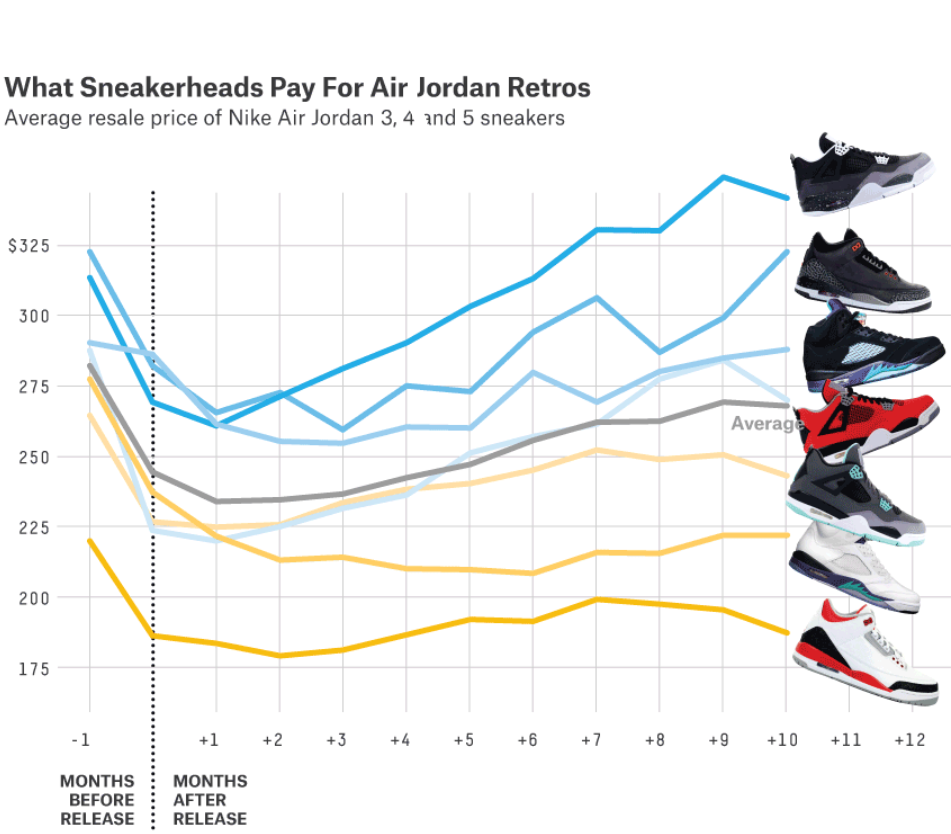
\includegraphics[width=0.6\columnwidth]{RealSneakersPrice.PNG}
    \caption{Price fluctuations of a specific sneaker over a one year period \cite{538} }
    \label{Jordans}
\end{figure}

The various simulations gave insight to the real market. Research into price fluctuations for sneakers revealed many graphs like \textit{Figure} \ref{Jordans}  which shows the price graph for "Air Jordan Retro" sneakers \cite{538}. 

It is also shown how this market behaves under nominal conditions that try to approximate the real world, and what would happen if some of the parameters of the model would change, and how can the different agents profit and use these changes for their own benefit.

\newpage
%\section{References}
\label{Bibliography}
\bibliographystyle{unsrtnat}
\bibliographystyle{538}
\bibliography{Bibliography}

\newpage
\appendix
\section{Appendix A}
\label{AppA}
\lstinputlisting[language=Matlab]{Financial_Model.m}
\end{document}  

